\chapter{Analisi del sistema \renuver{}}\label{chap:renuver}


\noindent Questo capitolo analizza il sistema oggetto di studio. L'analisi non si basa sulla
documentazione ma sul \emph{comportamento effettivo} del codice: il sistema è distribuito come
archivio eseguibile senza sorgenti, e le proprietà su cui poggia l'intera metodologia sono state
derivate per disassemblaggio. Ne emergono l'architettura e il flusso di imputazione, i ruoli che
le regole vi svolgono --- generazione dei candidati, verifica di coerenza e rivalutazione delle
regole escluse dalla ricerca ordinaria --- le due procedure con cui il sistema tratta le tuple
incomplete, e la distribuzione del costo computazionale fra le sue fasi. Da questa analisi
discendono le condizioni esatte di potatura su cui si fonda la metodologia, che sono esposte nel
capitolo successivo insieme alle strategie che le impiegano.

% =======================================================================================
\section{Obiettivi del sistema}\label{sec:renuver-goals}

\renuver{} \cite{breve2022renuver} è un algoritmo di imputazione di valori mancanti basato su
\emph{Relaxed Functional Dependencies}. L'idea portante è che le regole di imputazione non
debbano essere fornite dall'esterno, ma estratte dal dataset stesso: il sistema riceve in
ingresso un insieme di RFD già estratte e le impiega per ricostruire le celle nulle.

Rispetto ai metodi statistici, l'approccio ha il vantaggio di produrre imputazioni motivate da
vincoli osservati nei dati, e di poter \emph{rifiutare} di imputare quando nessun candidato
soddisfa i vincoli. Quest'ultima proprietà è deliberata: è preferibile una cella non imputata a
una cella imputata in violazione delle dipendenze del dataset.

% =======================================================================================
\section{Architettura generale}\label{sec:architecture}

\begin{figure}[htbp]
\centering
\begin{tikzpicture}[
    font=\footnotesize,
    box/.style={draw, rounded corners=1pt, align=center, inner sep=4pt, minimum height=8mm},
    file/.style={draw, align=center, inner sep=4pt, minimum height=8mm, fill=black!6},
    ar/.style={-{Latex[length=2mm]}, thick}
]
\node[file] (ds) {dataset\\$D$};
\node[box, right=8mm of ds] (est) {estrazione\\delle RFD};
\node[file, right=8mm of est] (rfd) {file delle\\regole $R$};
\node[box, right=8mm of rfd] (sys) {sistema\\\renuver{} };
\node[file, right=8mm of sys] (out) {celle\\popolate};
\node[box, below=10mm of rfd, fill=black!14] (prune) {potatura esterna\\(riscrittura del file)};
\draw[ar] (ds) -- (est);
\draw[ar] (est) -- (rfd);
\draw[ar] (rfd) -- (sys);
\draw[ar] (sys) -- (out);
\draw[ar] (ds.south) |- ([yshift=-4mm]sys.south) -- (sys.south);
\draw[ar] (rfd.south) -- (prune.north);
\draw[ar] (prune.east) -| ([xshift=6mm]sys.south);
\end{tikzpicture}
\caption{Flusso di elaborazione del sistema studiato e punto di innesto della potatura. La
potatura riscrive il file delle regole prima che il sistema lo consumi: il dataset e l'eseguibile
restano invariati.}
\label{fig:pipeline}
\end{figure}

Il sistema è distribuito come archivio Java eseguibile. L'analisi ha stabilito i seguenti fatti,
rilevanti per il seguito.

\begin{itemize}[leftmargin=1.4em]
    \item Il codice applicativo consta di \num{13} classi nel \emph{package} di default, incluse
    in un archivio ``grasso'' che incorpora anche la libreria di collezioni \texttt{fastutil}
    (\num{11040} classi complessive). Le classi applicative sono compilate per la versione
    \num{52} del formato \texttt{class} (Java~8).
    \item L'interfaccia a riga di comando accetta sei argomenti: la tipizzazione delle colonne,
    il file del dataset, il separatore, il file delle RFD, una soglia numerica e un selettore
    di euristica.
    \item \textbf{Il sesto argomento è ignorato.} Il metodo di avvio non lo legge: il sistema
    esegue sempre la medesima procedura di riempimento. Le altre procedure presenti nel codice
    --- ricerca locale, riordino per numero di valori nulli, riordino per coinvolgimento nel
    lato sinistro --- non sono raggiungibili dalla riga di comando. La verifica è stata condotta
    per disassemblaggio e confermata empiricamente. Il \texttt{README} dell'archivio documenta
    peraltro i parametri come \texttt{args0}--\texttt{args4} e \texttt{args6} --- l'indice
    \texttt{args5} non compare --- e precisa che ``in questa versione è supportata soltanto
    l'euristica sequenziale \texttt{0}'': la documentazione dichiara quindi un limite di
    \emph{versione}, mentre il codice mostra che l'argomento non viene mai letto. Le due
    circostanze sono distinte e la seconda è più forte della prima, perché esclude che il
    parametro possa essere onorato da una versione futura senza modifiche al codice.
    \item La quinta soglia ha un \emph{doppio ruolo}: filtra le RFD in ingresso e funge da
    valore iniziale della soglia di accettazione del punteggio di similarità. I due ruoli non
    sono separabili dalla riga di comando.
\end{itemize}

% =======================================================================================
\section{Flusso di imputazione e procedure di riempimento}\label{sec:workflow}\label{sec:two-branches}

Il flusso si articola in tre fasi.

\begin{enumerate}[leftmargin=1.6em]
    \item \textbf{Costruzione degli indici.} Le RFD vengono raggruppate in \emph{cluster},
    dove un cluster è l'insieme delle regole che condividono lo stesso attributo di destra e la
    stessa soglia di destra. Contestualmente si individuano le tuple del dataset che presentano
    celle nulle.
    \item \textbf{Trattamento delle tuple incomplete.} Per ogni tupla con celle nulle si tenta
    di riempirle, secondo due procedure distinte a seconda che la tupla abbia una sola cella
    nulla o più di una (\autoref{sec:two-branches}).
    \item \textbf{Verifica e registrazione.} Ogni imputazione candidata è sottoposta a una
    verifica di coerenza rispetto all'insieme delle regole; solo se supera la verifica viene
    registrata.
\end{enumerate}

% =======================================================================================
\section{Dataset impiegati}\label{sec:datasets}

L'archivio comprende cinque famiglie di dataset, con caratteristiche molto diverse fra loro. La
\autoref{tab:families} ne riassume la struttura rilevante per il pruning.

\begin{table}[htbp]
\centering
\caption{Caratteristiche delle famiglie di dataset. $N$ è il numero di RFD alla soglia indicata;
``celle valutate'' è il numero di celle per cui è disponibile il valore di ground truth, che
--- come si dirà --- non coincide con il numero di celle nulle del dataset.}
\label{tab:families}
\footnotesize
\begin{tabular}{lrrrr}
\toprule
famiglia & dataset & $N$ (soglia) & celle valutate & esito dell'analisi \\
\midrule
Bridges    & 25 & \num{1830}--\num{18844} & 14--70   & utilizzabile \\
Glass      & 25 & \num{1511}--\num{27445} & 22--107  & richiede correzione di schema \\
Restaurant & 45 & 25--124               & fino a \num{2074} & utilizzabile con metrica testuale \\
Physician  & 29 & \num{3734}            & fino a \num{338507} & non utilizzabile \\
Nursery    &  0 & \num{60}--\num{1693} byte & ---      & regole presenti, dataset assenti \\
\bottomrule
\end{tabular}
\end{table}

Due circostanze vanno segnalate perché condizionano la valutazione sperimentale.

\paragraph{Le celle valutate non sono le celle nulle.} Il valore di ground truth è fornito da un
file separato, in formato \texttt{riga;attributo;valore}, che elenca soltanto le celle introdotte
artificialmente. Il dataset può contenere altre celle nulle, preesistenti, che il sistema
tratta ma che non vengono valutate. Di conseguenza copertura e accuratezza sono relative
all'insieme delle celle elencate, non a tutte le celle nulle del dataset. La distinzione è
necessaria per interpretare correttamente le metriche.

\paragraph{Il costo computazionale non è uniforme.} I dataset Physician non remodulati contengono
\num{103592} righe e fino a \num{121913} celle nulle: una singola esecuzione richiederebbe tempi
non compatibili con una campagna sperimentale. Le versioni \emph{remodulate} della stessa
famiglia, di dimensioni ridotte, presentano a loro volta difetti nel materiale di ground truth
(\autoref{chap:defects}).

% =======================================================================================
\section{Il doppio ruolo delle RFD}\label{sec:dual-role}

\begin{algorithm}[htbp]
\caption{Verifica dei veti su una tupla incompleta, ricostruita dal bytecode. Il ciclo esamina
\emph{tutte} le regole dell'insieme e, per ciascuna, scansiona il dataset alla ricerca di un
testimone che violi la soglia di destra.}
\label{alg:veto}
\begin{algorithmic}[1]
\State \textbf{input}: tupla $t$ con la cella $t[A]$ nulla, insieme di regole $R$, dataset $D$
\ForAll{$r \in R$ tale che $\RHS(r) = A$}
    \If{$\LHS(r) \cap \NullCols(D) = \emptyset$}
        \State \textbf{continue} \Comment{nessun confronto possibile: la regola non può vetare}
    \EndIf
    \State cerca in $D$ una tupla $s \neq t$ che concordi con $t$ su ogni colonna di $\LHS(r)$
           entro la soglia $\theta_r$
    \If{esiste $s$ e $t[A]$ differisce da $s[A]$ oltre $\theta_{\RHS}(r)$}
        \State \Return \textbf{incoerente} \Comment{veto esercitato da $r$}
    \EndIf
\EndFor
\State \Return \textbf{coerente}
\end{algorithmic}
\end{algorithm}

Questa sezione stabilisce il vincolo che determina l'intero problema. L'analisi del codice mostra
che una RFD partecipa a \emph{due} procedure con requisiti opposti.

\begin{description}[leftmargin=0em]
    \item[Ruolo generativo.] Data una cella nulla, il sistema cerca tuple del dataset
    sufficientemente simili alla tupla incompleta; il punteggio di similarità è calcolato
    rispetto alle regole di un cluster, e il miglior punteggio determina il valore da imputare.
    In questo ruolo una soglia \emph{larga} rende la regola più permissiva.

    \item[Ruolo di veto.] Prima di registrare un'imputazione, il sistema verifica che essa non
    violi alcuna regola. In questo ruolo una soglia \emph{stretta} rende la regola più severa.
\end{description}

Le due procedure non sono separabili nel formato del file: una RFD è una riga di testo, e nulla
indica se essa serva all'una, all'altra, o a entrambe. Ne segue l'osservazione che governa il
lavoro.

\begin{observation}[Il pruning esterno è intrinsecamente conservativo]\label{obs:conservative}
Poiché rimuovere una regola ne elimina simultaneamente il contributo generativo e quello di veto,
e poiché i due contributi non sono distinguibili dal formato, una strategia di potatura che operi
sul solo file delle regole deve assumere che ogni regola rimossa possa essere necessaria al veto.
\end{observation}

La \autoref{tab:veto-share} quantifica quanto questa assunzione sia stringente: la quasi totalità
delle regole è, in linea di principio, in grado di esercitare un veto.

\paragraph{Un terzo ruolo, esercitato da una parte delle regole.} All'avvio il sistema compie una
propria riduzione dell'insieme: le regole con soglia di destra \emph{esattamente nulla} il cui lato
sinistro si comporta come una chiave sul dataset vengono tolte dall'insieme di lavoro, raccolte in
una struttura separata e sottoposte a una procedura distinta, invocata quando la ricerca ordinaria
di un candidato non produce alcun valore accettabile. Il log dell'esecuzione registra l'operazione
(``\texttt{Removing key RFD\ldots}''), e il numero di regole rimosse non è marginale: su
\texttt{bridges\_14\_1} a soglia 9 l'insieme passa da \num{8961} a \num{8581} regole. La verifica
della proprietà di chiave è inoltre quadratica nella dimensione del dataset, ed è la ragione per
cui il preprocessing del sistema --- che non è la potatura studiata in questo lavoro, ma una fase
interna dell'eseguibile --- domina il tempo sulle configurazioni grandi: sulla medesima
configurazione \SI{24.5}{\second} di preprocessing contro \SI{7.1}{\second} di imputazione, e fino
a \SI{113}{\second} su una configurazione Physician.

La circostanza ha due conseguenze. La prima riguarda la descrizione del sistema: i ruoli
osservabili sono \emph{tre}, non due, e il terzo è esercitato soltanto da una parte delle regole.
La seconda riguarda la portata delle garanzie: la condizione \Vtwo{} e il teorema del
\autoref{chap:theory} sono enunciati rispetto all'insieme delle regole così come compare nel file,
mentre il sistema ne consuma un sottoinsieme determinato da un criterio proprio; la verifica
sperimentale di equivalenza (\autoref{sec:res-vetocover}) copre l'interazione fra i due
meccanismi, ma un trattamento formale che la includesse dovrebbe modellare anche quella
riduzione. La questione è ripresa nella \autoref{sec:theory-scope}.

\begin{table}[htbp]
\centering
\caption{Quota di RFD che possono esercitare un veto, per famiglia e soglia. Una RFD può
esercitare un veto solo se il suo lato sinistro coinvolge almeno una colonna che presenta celle
nulle nel dataset.}
\label{tab:veto-share}
\footnotesize
\begin{tabular}{llrrr}
\toprule
famiglia & soglia & $N$ & RFD che \emph{possono} fare veto & quota \\
\midrule
Bridges    & 3  & \num{1830}  & \num{1818} & \SI{99.3}{\percent} \\
Bridges    & 9  & \num{8961}  & \num{8945} & \SI{99.8}{\percent} \\
Bridges    & 15 & \num{18844} & \num{18828} & \SI{99.9}{\percent} \\
Glass      & 3  & \num{1511}  & \num{1476} & \SI{97.7}{\percent} \\
Glass      & 9  & \num{11648} & \num{11564} & \SI{99.3}{\percent} \\
Glass      & 15 & \num{27445} & \num{27327} & \SI{99.6}{\percent} \\
Restaurant & 3  & 25          & 23         & \SI{92.0}{\percent} \\
Restaurant & 6  & 124         & 116        & \SI{93.5}{\percent} \\
\bottomrule
\end{tabular}
\end{table}

% =======================================================================================

\paragraph{Le due procedure di riempimento.} Il trattamento di una tupla incompleta segue due
procedure diverse, la cui distinzione è essenziale per interpretare i risultati.

\paragraph{Tupla con una sola cella nulla.} Il sistema scorre i cluster della colonna interessata
e si arresta al primo che produce un candidato valido. Esiste inoltre una scorciatoia: se la
regola impiegata ha soglia di destra nulla, il valore della tupla candidata viene scritto
direttamente e la procedura termina. Ne segue che, in questo ramo, la \emph{posizione} di un
cluster nell'ordine di scansione è determinante.

\paragraph{Tupla con più celle nulle.} La procedura è iterativa: per un numero di round pari al
massimo numero di cluster fra le colonne coinvolte, e per ciascun round, ogni cella nulla riceve
i candidati del cluster corrispondente al round corrente. La scrittura del valore avviene senza
verificare se la cella sia già stata riempita in un round precedente; un round successivo
sovrascrive quindi il risultato del precedente, e un round i cui candidati fallissero tutti la
verifica di coerenza può riportare la cella allo stato nullo. In questo ramo, dunque, il valore
finale di una cella dipende dall'\emph{ultimo} cluster produttivo della sua colonna.

La distinzione ha una conseguenza quantitativa che sarà ripresa nel \autoref{chap:results}: le
due procedure non sono ugualmente rappresentate nei dataset. Su Bridges circa tre quarti delle
celle nulle appartengono a tuple con più di una cella nulla, mentre su Glass e Restaurant la
grande maggioranza appartiene a tuple con una sola cella nulla.

% =======================================================================================
\section{Costo computazionale}\label{sec:cost}

\begin{figure}[htbp]
\centering
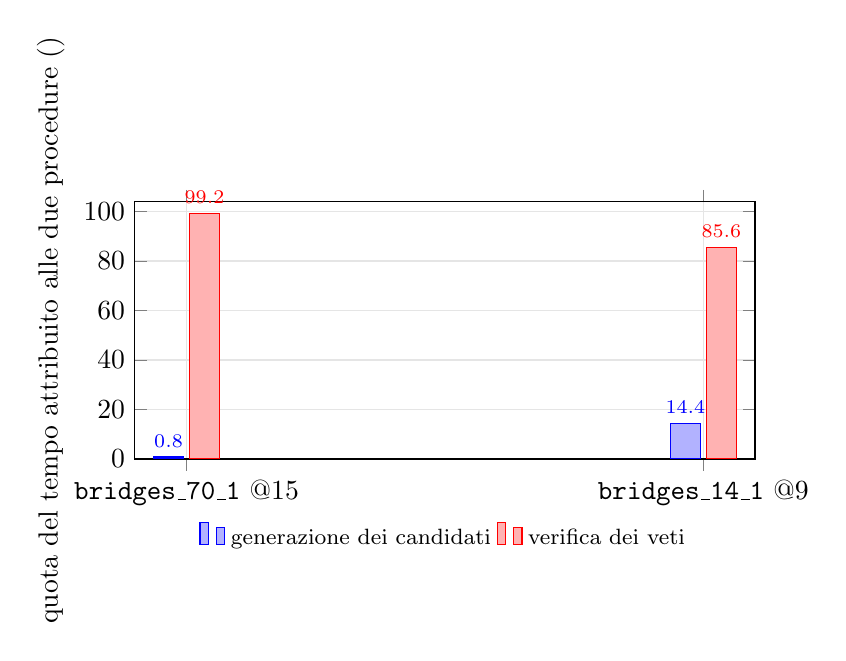
\begin{tikzpicture}
\begin{axis}[
    ybar,
    bar width=11pt,
    width=0.78\textwidth,
    height=0.40\textwidth,
    ymin=0, ymax=104,
    ylabel={quota del tempo attribuito alle due procedure (\si{\percent})},
    xtick={1,2},
    xticklabels={\texttt{bridges\_70\_1} @15, \texttt{bridges\_14\_1} @9},
    legend style={font=\footnotesize, at={(0.5,-0.22)}, anchor=north, legend columns=2, draw=none, fill=none},
    nodes near coords,
    every node near coord/.append style={font=\scriptsize},
    grid=major,
    grid style={black!10},
]
\addplot coordinates {(1,0.8) (2,14.4)};
\addplot coordinates {(1,99.2) (2,85.6)};
\legend{generazione dei candidati, verifica dei veti}
\end{axis}
\end{tikzpicture}
\caption{Ripartizione del tempo di esecuzione fra le due procedure, misurata per strumentazione su
due configurazioni. La verifica dei veti domina in entrambe, e all'interno di essa il costo è
quasi interamente nella scansione del dataset.}
\label{fig:cost}
\end{figure}

Poiché il sistema è distribuito senza sorgenti, la determinazione di dove si concentri il tempo
di esecuzione richiede di ricompilarlo e strumentarlo. La procedura --- ricompilazione da sorgenti
decompilati, con verifica di equivalenza rispetto all'eseguibile originale --- è descritta
nella \autoref{sec:instrumentation}; qui se ne riportano i risultati, che orientano la scelta delle
strategie di ottimizzazione.

\begin{table}[htbp]
\centering
\caption{Ripartizione del tempo di esecuzione fra le due procedure principali, misurata per
strumentazione. La percentuale è calcolata sul tempo complessivamente attribuito alle due
procedure.}
\label{tab:cost}
\footnotesize
\begin{tabular}{lrrrr}
\toprule
configurazione & procedura & chiamate & tempo & quota \\
\midrule
\multirow{2}{*}{\texttt{bridges\_70\_1}, soglia 15}
  & generazione candidati & 531      & \SI{1.4}{\second}   & \SI{0.8}{\percent} \\
  & verifica dei veti     & 151      & \SI{158.4}{\second} & \SI{99.2}{\percent} \\
\midrule
\multirow{2}{*}{\texttt{bridges\_14\_1}, soglia 9}
  & generazione candidati & 293      & \SI{1.5}{\second}   & \SI{14.4}{\percent} \\
  & verifica dei veti     & 8        & \SI{9.1}{\second}   & \SI{85.6}{\percent} \\
\bottomrule
\end{tabular}
\end{table}

All'interno della verifica dei veti, la quasi totalità del tempo è assorbita dalla scansione del
dataset: su \texttt{bridges\_70\_1} a soglia 15, \num{354809} invocazioni della verifica di
violazione assorbono \SI{158.3}{\second} su \SI{158.4}{\second} totali, mentre il confronto dei
nomi di colonna --- che pure è il primo test eseguito --- costa \SI{0.16}{\second}.

Il risultato ha una conseguenza diretta e controintuitiva: \textbf{il tempo è nel veto, non nella
generazione}. Ne segue che le strategie di potatura producono un guadagno temporale proprio in
quanto riducono il numero di regole esaminate dalla verifica dei veti, e che qualunque
ottimizzazione mirata alla sola generazione dei candidati non potrebbe che incidere su una
frazione marginale del costo.

